\documentclass[10pt,a4paper]{article}
\usepackage[T1]{fontenc}
\usepackage{mathptmx}
\usepackage[margin=1in]{geometry}
\usepackage{graphicx}
\usepackage{booktabs}
\usepackage{array}
\usepackage{float}
\usepackage{amsmath}
\usepackage[hidelinks]{hyperref}
\usepackage{enumitem}
\usepackage{caption}
\usepackage{microtype}
\usepackage{tikz}
\usetikzlibrary{arrows.meta,positioning}
\usepackage[numbers,sort&compress]{natbib}
\captionsetup{font=small,labelfont=bf}
\setlist{itemsep=1pt,topsep=3pt}
\graphicspath{{../analysis/output/}}

\title{\textbf{Filling the Gaps: How Often Do LLM Agents Misreport\\ Figures When They Build Financial Models?}}
\author{Joaquim Manji-Jung\\[2pt]
\small Paris, France\\
\small \href{https://github.com/joaquimmj/deskstack}{github.com/joaquimmj/deskstack}}
\date{November 2026}

\begin{document}
\maketitle

\begin{abstract}
\noindent When an LLM agent builds a financial model, every historical figure in it should come from the company's
filings. We measure how often it does not. In a benchmark of 300 runs, Claude Sonnet 5.5 built a discounted cash
flow (DCF) model and a trading-comparables table for each of 50 listed companies (35 US, 15 European) under three
conditions: with web search only (A), with tools that return figures read from SEC and ESEF filings (B), and with
the same tools plus an automated review round (C). Every figure the scorer flagged was then checked by hand against
the filing. With web search only, 3.5\% of filed figures were wrong (36 of 1{,}018; 95\% CI 2.6--4.9\%), and 24\%
of DCF models contained at least one wrong figure. With sourced data, none of 3{,}230 figures was wrong (exact
95\% upper bound 0.11\%), at about a third of the cost. Most web-search errors were not misreadings but
\emph{substitutions}: when the agent could not find a figure, it wrote an estimate, a non-GAAP or aggregator number,
or the right figure for the wrong period, often while noting the doubt in its own source notes. A pre-registered
robustness check found that the errors persist with 2.5$\times$ the search budget and higher reasoning effort.
Before the hand reading, the automated scorer overstated the error rate by 2.5$\times$; we report how, because it
bears on how such agents should be evaluated. We release all prompts, transcripts, scores, hand readings and the
analysis code.
\end{abstract}

\section{Introduction}

Language models increasingly do analytical work end to end: an agent is asked for a valuation, searches for inputs,
and returns a finished spreadsheet. The failure that matters most in that setting is not an obviously broken model
but a plausible one with a few wrong inputs. A share count off by a quarter, or revenue a quarter stale, does not
break any formula; it silently moves the answer, and a reviewer has no signal that it happened unless they tie every
figure back to the filing.

This is a specific, measurable instance of a general problem: a model that cannot find a fact tends to produce a
plausible one rather than abstain \citep{ji2023,kalai2025}. Financial filings make it unusually easy to measure,
because the ground truth is public, structured (XBRL in the US, ESEF in Europe) and unambiguous for most reported
lines. Existing financial benchmarks test question answering over documents the model is given
\citep{chen2021finqa,islam2023financebench}; we instead test an agent that must \emph{find} its inputs, as it would
in practice, and we score every figure it reports. Grounding generation in retrieved sources is a standard remedy
\citep{lewis2020}; we measure how much it buys when the source is the filing itself.

We ask three questions:
\begin{enumerate}
  \item How often does an agent with web search write a historical figure that differs from the filing?
  \item Does giving it tools that return sourced figures remove those errors, and at what cost?
  \item Do the errors go away if the agent is simply given more search budget and reasoning effort?
\end{enumerate}

\paragraph{Contributions.} (i) A benchmark of 300 agent runs on two standard finance tasks, scored figure by figure
against the filings, with every flagged figure read by hand. (ii) A measured error rate for web search alone, and the
finding that sourced-data tools remove it at lower cost. (iii) A taxonomy of the errors, which shows they are
substitutions rather than misreadings, and that the agent often knew. (iv) A pre-registered test showing that more
search and more effort do not remove them. (v) A measurement of the automated scorer itself, whose precision on
arm A was 40--57\%, a caution for anyone evaluating agents with an automatic oracle alone.

\section{Related work}

\paragraph{Financial question answering.} FinQA \citep{chen2021finqa}, TAT-QA \citep{zhu2021tatqa} and ConvFinQA
\citep{chen2022convfinqa} test numerical reasoning over tables and text taken from reports; FinanceBench
\citep{islam2023financebench} asks open questions about public filings and finds that retrieval set-ups often fail
on them. In all of these the evidence is given or retrieved by a fixed pipeline, and the answer is a single number or
sentence. Our agents choose their own sources and produce dozens of figures per model, and we score all of them.

\paragraph{Factuality and abstention.} Hallucination is surveyed by \citet{ji2023}. Fine-grained factuality metrics
such as FActScore \citep{min2023factscore} score each atomic claim of a long answer against a knowledge source; we do
the same for numbers, with the filing as the source. Models can often estimate whether they know an answer
\citep{kadavath2022}, and \citet{kalai2025} argue that standard training and evaluation reward guessing over
abstaining. Our finding that the agent flagged its own doubts in notes but still used the number is an instance of
that gap, in an agentic setting.

\paragraph{Tool use and retrieval.} Agents that interleave reasoning with tool calls \citep{yao2023react,schick2023}
and retrieval-augmented generation \citep{lewis2020} are the standard way to ground outputs. We compare two kinds of
grounding: open web search, and tools that return figures already tied to a filing, an accession number and a
period.

\paragraph{Scalable oversight.} Checking a long agent output is costly for a human, which motivates work on scalable
oversight \citep{bowman2022}. Our results bear on one design choice in that space: constraining what inputs the agent
can use, rather than checking its outputs afterwards.

\section{Method}

\begin{figure}[htb]
\centering
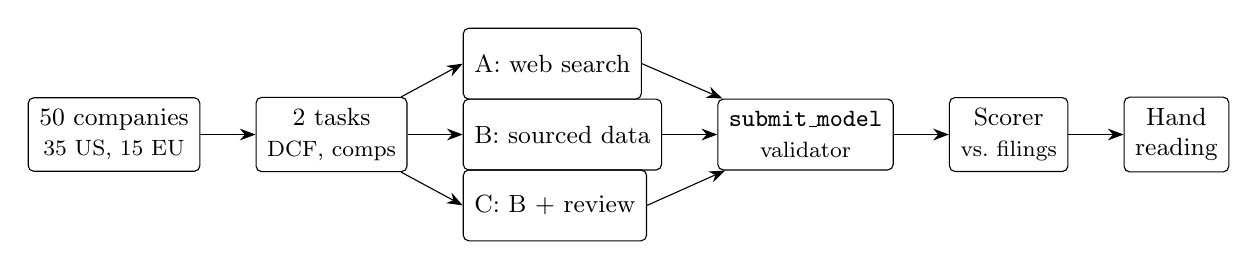
\begin{tikzpicture}[
  node distance=4mm and 7mm,
  box/.style={draw, rounded corners=2pt, align=center, font=\small, inner sep=4pt, minimum height=9mm},
  arr/.style={-{Stealth[length=2mm]}, thin}]
\node[box] (co) {50 companies\\ \footnotesize 35 US, 15 EU};
\node[box, right=of co] (task) {2 tasks\\ \footnotesize DCF, comps};
\node[box, right=of task, yshift=9mm] (a) {A: web search};
\node[box, right=of task] (b) {B: sourced data};
\node[box, right=of task, yshift=-9mm] (c) {C: B + review};
\node[box, right=of b] (sub) {\texttt{submit\_model}\\ \footnotesize validator};
\node[box, right=of sub] (sc) {Scorer\\ \footnotesize vs.\ filings};
\node[box, right=of sc] (hand) {Hand\\ reading};
\draw[arr] (co) -- (task);
\draw[arr] (task) -- (a.west); \draw[arr] (task) -- (b); \draw[arr] (task) -- (c.west);
\draw[arr] (a.east) -- (sub); \draw[arr] (b) -- (sub); \draw[arr] (c.east) -- (sub);
\draw[arr] (sub) -- (sc); \draw[arr] (sc) -- (hand);
\end{tikzpicture}
\caption{Benchmark design. Each of 100 company-tasks is run in three arms that differ only in the tools; every
submission is scored against the filings, and every figure the scorer calls wrong is read by hand.}
\label{fig:design}
\end{figure}

\paragraph{Company set.} 50 non-financial companies (35 US, 15 EU) in 36 sectors, frozen before any run
(Appendix~\ref{app:companies}). The set deliberately includes awkward cases: fiscal years ending in January, May,
September, October and November, 52/53-week years, a company with losses, a dual filer (ASML, US GAAP 20-F and IFRS
report) and an industrial conglomerate. Banks and insurers are excluded because an unlevered DCF does not apply to them. A
5-company pilot was run first; it led to two new scoring categories and five data fixes, and is not part of the
results.

\paragraph{Tasks.} Each company gets two tasks, built from scratch: (i) a quick DCF, whose filed inputs are the
historical income-statement and cash-flow lines, net debt and diluted shares; and (ii) a comps table of the company
and 4--6 listed peers the agent picks, with revenue, EBITDA, net income, net debt and market capitalisation, each
with its source and period. A comps table is ``as of now'', so its figures are the last twelve months available.

\paragraph{Arms.} All arms use \texttt{claude-sonnet-5-5} at medium effort with the same frozen prompts (v2), which
fix conventions (sign of capex, EBITDA and net-debt definitions) so that only the tools differ.
\begin{itemize}
  \item \textbf{A, web search only:} up to 12 searches per request. A model that runs out can still submit; figures
        it leaves as labelled placeholders are counted apart.
  \item \textbf{B, sourced data:} tools that return figures read from SEC \texttt{companyfacts} and ESEF reports, each
        with its source (filing, accession or report, period). B also receives the tool server's instructions, as
        real clients of such a server do.
  \item \textbf{C, sourced data + review:} B, then one review round and a fix. The review is a tie-out of every filed
        figure against the filing and the findings of a deterministic model checker.
\end{itemize}
Every arm submits the same structured model through one tool, whose validator rejects missing sources, rates typed
as percents and WACC $\le g$, and returns the errors to the agent to fix.

\paragraph{Scoring.} Scoring is automatic and against the filings, with no human grading of quality. A reported
figure is \emph{wrong} if it differs from the filed value for the period asked and matches no other line of the same
filing. Figures equal to another line (e.g.\ revenue excluding excise taxes) are reported as \emph{other line};
EBITDA and net debt, which depend on a definition, as \emph{other definition}; lines the filing does not report for
that period, or peers that cannot be resolved by name, as \emph{not verifiable}. None of these count as wrong. Peers
with colliding tickers (MC is LVMH in Paris and Moelis in New York) are never scored against the wrong company.

\paragraph{Hand reading.} Every figure the scorer still called wrong was read by hand against the filing. This
matters: the scorer's precision on arm A was 40\% for DCFs (20 of 50 flags were real errors) and 57\% for comps
(16 of 28). The rest were the scorer's or the data's limitations (\S\ref{sec:scorer}). All numbers below are after
the hand reading.

\paragraph{Budget control.} Every request is priced at its worst case before it is sent (all input billed as a cache
write, full output, every allowed search) and refused if it could cross a hard cap recorded in a ledger. The SDK's
own retries are off, and only non-billed overload errors are retried, so the spend reported is the spend incurred.

\paragraph{Statistics.} Proportions are reported with Wilson 95\% intervals, zero counts with exact Clopper--Pearson
intervals, and differences with Newcombe's hybrid score interval \citep{wilson1927,clopper1934,newcombe1998}. Arm
comparisons use Fisher's exact test, the two tasks are pooled with a Cochran--Mantel--Haenszel test, and DCF arms are
compared at the company level with an exact McNemar test. Because errors cluster within companies, we also bootstrap
the arm-A DCF rate over companies (20{,}000 resamples, fixed seed). The analysis is in
\texttt{bench/analysis/analyze.py}.

\section{Results}

\begin{table}[htb]
\centering
\small
\begin{tabular}{llrrrrrr}
\toprule
Task & Arm & Wrong / checked & Rate & 95\% CI & Cost & Tokens & Time \\
\midrule
DCF   & A: web search      & 20 / 573   & 3.49\% & 2.27--5.33\% & \$0.23 & 152k & 58 s \\
      & B: sourced data    & 0 / 593    & 0      & 0--0.62\%    & \$0.07 & 38k  & 18 s \\
      & C: sourced + review& 0 / 606    & 0      & 0--0.61\%    & \$0.10 & 69k  & 32 s \\
\midrule
Comps & A: web search      & 16 / 445   & 3.60\% & 2.23--5.76\% & \$0.55 & 601k & 167 s \\
      & B: sourced data    & 0 / 1{,}021& 0      & 0--0.36\%    & \$0.17 & 126k & 36 s \\
      & C: sourced + review& 0 / 1{,}010& 0      & 0--0.36\%    & \$0.22 & 202k & 51 s \\
\bottomrule
\end{tabular}
\caption{Wrong filed figures, read by hand, with average cost, tokens and time per model. Intervals: Wilson for
non-zero counts, exact for zeros. Comps are counted over the 49 companies where every arm finished.}
\label{tab:main}
\end{table}

\begin{figure}[htb]
\centering
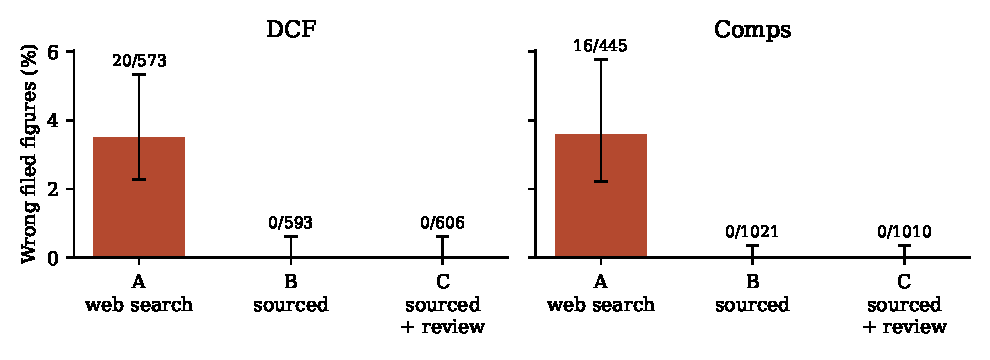
\includegraphics[width=0.82\linewidth]{fig_error_rates.pdf}
\caption{Share of filed figures that are wrong, by arm, with 95\% intervals.}
\label{fig:rates}
\end{figure}

\paragraph{Web search alone gets about one figure in 28 wrong.} Table~\ref{tab:main} and Figure~\ref{fig:rates}
give the main result. Pooled over both tasks, arm A wrote 36 wrong figures out of 1{,}018 checked (3.54\%; 95\% CI
2.57--4.86\%). The rate is almost identical across the two tasks (3.49\% and 3.60\%), although the causes differ.
Arm A also left 7 comps figures as labelled zeros (``not found, 0 is a placeholder''); they are not counted as wrong,
but any ratio computed from them is.

\paragraph{The errors are concentrated, but common at the model level.} In the DCF task, 12 of 50 models (24\%;
95\% CI 14--37\%) contained at least one wrong figure. Errors cluster: the three worst companies hold half of them
(Cisco 4, GE Aerospace 3, Stellantis 3). Bootstrapping over companies widens the interval on the arm-A rate to
1.6--5.8\% (design effect 2.0). Because the committed summaries do not give figures per company, the bootstrap spreads
checked figures evenly; letting them vary at random moves the bounds by less than half a percentage point.

\paragraph{Sourced data removes them, at a third of the cost.} Neither arm B nor arm C wrote a wrong figure in
3{,}230 checked (exact 95\% upper bound 0.11\%). Against arm A the difference is 3.5 percentage points in each task
(Newcombe 95\% CI 2.1--5.3 for DCF, 2.2--5.8 for comps; Fisher $p<10^{-6}$ in every comparison). Pooled across tasks,
the CMH test gives $\chi^2 = 102.5$, $p \approx 4\times10^{-24}$. At the company level, the exact McNemar test gives
$p = 9.8\times10^{-4}$ for A against B, computed conservatively as if B's one unfinished run were among A's twelve
error companies, and $p = 4.9\times10^{-4}$ for A against C.

\begin{figure}[htb]
\centering
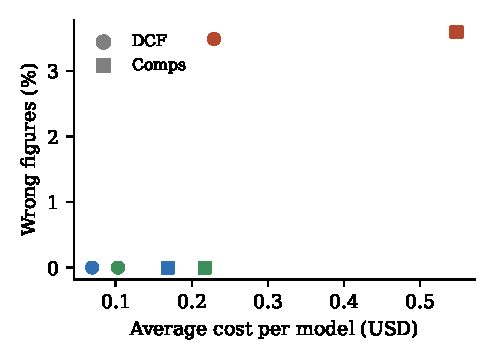
\includegraphics[width=0.55\linewidth]{fig_cost_accuracy.pdf}
\caption{Accuracy against cost per model. Red: arm A; blue: arm B; green: arm C. Sourced data is both cheaper and
more accurate, in both tasks.}
\label{fig:cost}
\end{figure}

\paragraph{Cheaper and faster, because pages stay out of context.} Arm B cost 0.30--0.31$\times$ arm A and ran
3--5$\times$ faster (Figure~\ref{fig:cost}). The difference is mostly input tokens: an agent with web search reads
whole pages into its context, 152k tokens per DCF and 601k per comps table on average, against 38k and 126k for arm
B. Web search is also billed per search. Of the comps spend, arm A accounted for \$27.81, arm B \$8.44 and arm C
\$10.84.

\paragraph{Completion.} Arm A finished 50 of 50 DCFs and 45 of 50 comps tables: one run timed out, and in four the
validator rejected a missing market capitalisation and the agent stopped instead of fixing it. Arm B finished 49 of
50 DCFs and all comps; arm C finished every run.

\paragraph{Review added little to accuracy here.} Arm C matched arm B, since B already had no wrong figures to
correct. The review's measurable effect was on model quality: the deterministic checker's major findings per DCF fell
from 0.63 (B) to 0.36 (C), against 0.66 for A; no arm had a blocker. This benchmark cannot separate the value of
review from the value of sourced data, because the latter already reaches the floor.

\paragraph{Provenance is a separate question.} The share of typed numbers with no source (missing, a placeholder,
or ``not found'') was 7.1\% (A), 4.4\% (B) and 4.7\% (C) in DCFs, but 11.9\%, 17.1\% and 16.8\% in comps. We did not
read these by hand. They measure whether a figure carries a citation, not whether it is right, and the higher comps
share in B and C shows that sourced tools do not by themselves make an agent cite everything it types.

\section{What the errors are}

\begin{figure}[htb]
\centering
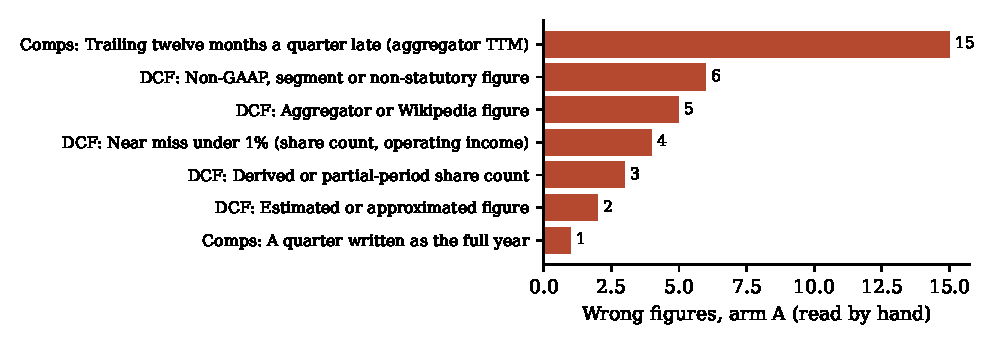
\includegraphics[width=0.9\linewidth]{fig_error_causes.pdf}
\caption{Causes of arm A's 36 wrong figures, each read by hand against the filing.}
\label{fig:causes}
\end{figure}

\begin{table}[htb]
\centering
\small
\begin{tabular}{>{\raggedright\arraybackslash}p{3.9cm}r>{\raggedright\arraybackslash}p{9.7cm}}
\toprule
Cause & $n$ & Examples (written value against filed value, millions) \\
\midrule
TTM a quarter late (comps) & 15 & Motorola Solutions revenue 12{,}240, the twelve months to June (12{,}236), when the
September 10-Q was filed; Fortinet 7{,}530 likewise; FedEx's fiscal year to May used as LTM \\
Quarter written as the year & 1 & Boeing net income: the fourth quarter (8{,}220) as the full year (2{,}235) \\
Non-GAAP, segment, non-statutory & 6 & GE Aerospace adjusted revenue ($\times$2); Stellantis D\&A of industrial
activities, not the group ($\times$3); Iberdrola ``gross investment'' as capex \\
Aggregator or Wikipedia & 5 & Cisco ($\times$3) and Verizon operating income from data sites; Schneider Electric
operating income, rounded, from Wikipedia \\
Derived share count & 3 & Boeing, Pfizer and GE Aerospace diluted shares: net income / EPS, six months, Q1 \\
Estimated & 2 & Netflix capex as operating cash flow minus free cash flow; UPS revenue from nine months plus a
rounded fourth quarter \\
Near miss under 1\% & 4 & Share counts or operating income (Chevron, Cisco, UPS, Thermo Fisher) \\
\bottomrule
\end{tabular}
\caption{The 36 wrong figures in arm A, by cause, with examples from the hand reading.}
\label{tab:causes}
\end{table}

Figure~\ref{fig:causes} and Table~\ref{tab:causes} classify the 36 wrong figures. Almost none is a misreading of a
source the agent had found. They are substitutions: the agent needed a number, did not find the filed one, and wrote
something else.
\begin{itemize}
  \item \textbf{Stale periods (15 of 16 comps errors).} The agent took ``trailing twelve months'' figures from one
        aggregator, which still showed the twelve months to June 2026 when the September 10-Qs were filed. Each figure
        was right for an earlier period, which makes it the hardest kind of error for a reviewer to see.
  \item \textbf{Proxies and non-statutory figures (DCF).} Adjusted (non-GAAP) revenue, a segment's D\&A for the
        group's, a ``gross investment'' figure for capex.
  \item \textbf{Aggregators and Wikipedia (DCF).} Operating income from data sites or a rounded encyclopedia figure.
  \item \textbf{Derived or estimated numbers (DCF).} A share count computed as net income over EPS, a six-month or
        first-quarter count used for the year, capex estimated as operating cash flow minus free cash flow.
\end{itemize}
In about half of the DCF cases the agent said so in its own source notes (``reviewer should replace''), but the
number still went into the model and into the valuation. The model knew the figure was uncertain, and the output
did not show it. We think that gap matters for oversight: an agent's caveats are only useful if they change what it
outputs, or if a reviewer reads them.

\section{Robustness: is it just the search budget?}

The obvious objection is that arm A was starved of searches. We pre-registered a check before running it: on 10
companies (the 5 where arm A had erred in comps, plus 5 controls chosen by a fixed rule), the comps task was re-run at
12 searches and medium effort (A12, a fresh run of the main setting, since the model is not deterministic) and at 30
searches and high effort (A30). The stated reading rule was that if A30 had no wrong figures and no placeholders, we
would say the errors depend on the search budget; otherwise that they persist.

A30 still wrote a figure that was not the filing's: Chevron's net income as the model's own estimate (nine months
from the 10-Q plus ``about'' the fourth quarter: 12{,}329 against 12{,}299 filed). A12's error was Cigna's revenue
taken from an aggregator's rounded ``\$274.95B''. Wrong figures were 1 of 86 (A12) and 1 of 117 (A30), with no
detectable difference (Fisher $p = 1.0$). At the main comps rate, the chance of seeing no error in 117 figures would
be 1.4\%. More budget did remove the placeholders (7 to 0), at 2.3$\times$ the cost per table (\$1.59 against
\$0.68). By the pre-registered rule, the errors persist. The sample is small: this answers \emph{whether} the errors
go away with more search (no), not \emph{how often} they occur.

One amendment was made, and recorded, before any re-run: 7 of the 10 A30 runs hit the runner's \$3 per-run cost
cap, a property of our harness rather than of web search, and were re-run with a \$6 cap.

\section{Measuring the scorer}
\label{sec:scorer}

An automatic oracle is attractive for agent evaluation, so we report how far ours could be trusted. At run time the
scorer flagged 23 wrong DCF figures in arm A and one each in B and C, and 38, 10 and 8 in comps. Reading every flag
changed those numbers in both directions.

\begin{table}[htb]
\centering
\small
\begin{tabular}{>{\raggedright\arraybackslash}p{10.2cm}rr}
\toprule
Scorer flag on arm A, after rescoring, read by hand & DCF & Comps \\
\midrule
Real error: not the filed figure for the period asked & 20 & 16 \\
Placeholder 0, labelled as not found & -- & 7 \\
Another line of the company's own statements (e.g.\ Exxon ``sales and other operating revenue'') & 10 & 4 \\
Narrower line in the data (D\&A as depreciation only) & 9 & -- \\
Other accounting basis (ASML's US GAAP 20-F against its IFRS report) & 6 & -- \\
Company's own segment tag; the model was right (Disney operating income) & 3 & -- \\
Rounding, or results release against annual report & 1 & 1 \\
Filing's XBRL tag off by a factor of a million (McDonald's diluted shares) & 1 & -- \\
\midrule
Total flags & 50 & 28 \\
\bottomrule
\end{tabular}
\caption{What the scorer's flags on arm A turned out to be. Precision: 40\% (DCF), 57\% (comps).}
\label{tab:scorer}
\end{table}

\paragraph{Two scorer bugs, in both directions.} The ``other line'' rule first accepted any two lines of a filing
that added up to the submitted value; with hundreds of lines per filing, pairs matched by chance, and arm A's DCF
mismatches rose from 23 to 50 once lines had to belong to the metric's family. In comps, peers were matched by name
too loosely: Coca-Cola Europacific Partners was scored as Coca-Cola, and General Motors as GM Financial. Every one of
B's and C's flags, and 12 of A's, came from this. Table~\ref{tab:scorer} shows what the remaining flags were.

\paragraph{What it found in the data.} The reading also found and fixed four limitations of the data tools, none of
which changes a counted error: D\&A as depreciation only for filers that tag the two separately, Disney's tagged
segment total used as operating income, McDonald's share count tagged a million times too small since FY2023, and dual
filers whose US GAAP 20-F differs from their IFRS report.

The lesson is general. Without the hand reading, the DCF error rate of arm A would have been overstated by
2.5$\times$, and arms B and C would have shown errors they did not make. Automated scoring of agent output is a
screening step, not a measurement.

\section{Threats to validity}

\begin{itemize}
  \item \textbf{The oracle shares data with arms B and C.} The scorer checks figures with the same filing reader that
        B and C use, so their zero is partly by construction. That reader is checked independently: a hand-built
        golden set (99/99 at the time of the runs) and a nightly differential against two other XBRL parsers. The
        comparison that matters is A against B and C, and the scoring of A does not depend on the reader being right,
        because every A error was read by hand.
  \item \textbf{Not everything is scored.} EBITDA and net debt (definition-dependent), market caps and lines the
        filing does not report were not counted as wrong. Arm A had more such figures (87 \emph{not verifiable} DCF
        figures against 24 and 16), so if anything its true error rate is understated.
  \item \textbf{One model, one prompt version.} Results are for Claude Sonnet 5.5 at medium effort. Other models,
        stronger search tools or prompts that require abstention may behave differently.
  \item \textbf{Clustering.} Figures are not independent; the company-level tests and the bootstrap address this for
        the DCF task. For comps, peers are shared across tables, so the figure-level intervals are too narrow.
  \item \textbf{Timing.} The comps errors depend on when the runs happened: shortly after a filing season, when
        aggregators lag. Runs at another point in the quarter would likely see fewer stale periods and could see
        others.
  \item \textbf{One annotator.} The hand reading was done by the author. Each judgement is written down with the
        filing line it rests on, so it can be checked, but it was not double-coded.
\end{itemize}

\section{Discussion}

\paragraph{For practitioners.} An agent-built model with web inputs should be tied out figure by figure before it
is used. The errors are not random noise that averages out: a stale quarter or a non-GAAP revenue figure moves a
valuation in one direction, and a comps table with one late peer changes the median multiple. Because a quarter of
DCF models had at least one such figure, sampling a few models for review is not enough.

\paragraph{For evaluation design.} Our automated scorer was precise enough to screen but not to measure. Benchmarks
that report error rates from an automatic oracle alone should report its precision on a hand-read sample, as we do
in Table~\ref{tab:scorer}.

\paragraph{For oversight.} The agent's notes contained the right warning about half the time. An agent that abstains,
or that refuses to submit a figure it marked as uncertain, would turn those notes into a visible gap rather than a
silent error. Testing prompts and tools that enforce this is the natural next experiment.

\paragraph{Future work.} Other models and providers; prompts that require abstention; a run at mid-quarter to
separate staleness from search; banks and insurers with a dividend-discount task; and a second annotator.

\section{Conclusion}

An LLM agent with web search builds financial models that are mostly right and occasionally, silently, wrong: about
3.5\% of filed figures and a quarter of DCF models. The errors are substitutions for figures it could not find, they
survive more search and more effort, and the agent often flags them in notes that do not reach the output. Giving the
agent sourced data removes them in this benchmark and costs less. The broader lesson is about where to put
verification: checking an agent's outputs after the fact is expensive and, as our own scorer showed, error-prone;
constraining its inputs to sources that can be checked is cheaper and more reliable. As agents take on longer tasks,
that kind of design choice is one practical lever for keeping their work overseeable \citep{bowman2022}.

\paragraph{Reproducibility.} The company set, prompts, runner, scorer, summaries, hand readings
(\texttt{ANALYSIS.md} in each results folder), the pre-registration (\texttt{bench/ROBUSTNESS.md}) and this analysis
are in the repository; raw transcripts are archived on a GitHub release with a SHA-256 checksum. API spend for the runs
reported here was \$86.89 (DCF \$20.03, comps \$47.09, robustness \$19.77), plus \$6.68 for the pilot.

\paragraph{Acknowledgements.} The author used Claude (Anthropic) to help write the benchmark code, the statistical
analysis and the text of this paper. The author designed the study, checked every result and takes full
responsibility for the content.

{\small
\begin{thebibliography}{20}\setlength{\itemsep}{1pt}
\bibitem[Bowman et al.(2022)]{bowman2022} S.~R. Bowman et al. Measuring progress on scalable oversight for large
language models. \emph{arXiv:2211.03540}, 2022.
\bibitem[Chen et al.(2021)]{chen2021finqa} Z.~Chen et al. FinQA: A dataset of numerical reasoning over financial
data. In \emph{EMNLP}, 2021.
\bibitem[Chen et al.(2022)]{chen2022convfinqa} Z.~Chen et al. ConvFinQA: Exploring the chain of numerical reasoning
in conversational finance question answering. In \emph{EMNLP}, 2022.
\bibitem[Clopper and Pearson(1934)]{clopper1934} C.~J. Clopper and E.~S. Pearson. The use of confidence or fiducial
limits illustrated in the case of the binomial. \emph{Biometrika}, 26(4):404--413, 1934.
\bibitem[Islam et al.(2023)]{islam2023financebench} P.~Islam et al. FinanceBench: A new benchmark for financial
question answering. \emph{arXiv:2311.11944}, 2023.
\bibitem[Ji et al.(2023)]{ji2023} Z.~Ji et al. Survey of hallucination in natural language generation. \emph{ACM
Computing Surveys}, 55(12), 2023.
\bibitem[Kadavath et al.(2022)]{kadavath2022} S.~Kadavath et al. Language models (mostly) know what they know.
\emph{arXiv:2207.05221}, 2022.
\bibitem[Kalai et al.(2025)]{kalai2025} A.~T. Kalai, O.~Nachum, S.~S. Vempala and E.~Zhang. Why language models
hallucinate. \emph{arXiv:2509.04664}, 2025.
\bibitem[Lewis et al.(2020)]{lewis2020} P.~Lewis et al. Retrieval-augmented generation for knowledge-intensive NLP
tasks. In \emph{NeurIPS}, 2020.
\bibitem[Min et al.(2023)]{min2023factscore} S.~Min et al. FActScore: Fine-grained atomic evaluation of factual
precision in long form text generation. In \emph{EMNLP}, 2023.
\bibitem[Newcombe(1998)]{newcombe1998} R.~G. Newcombe. Interval estimation for the difference between independent
proportions: comparison of eleven methods. \emph{Statistics in Medicine}, 17(8):873--890, 1998.
\bibitem[Schick et al.(2023)]{schick2023} T.~Schick et al. Toolformer: Language models can teach themselves to use
tools. In \emph{NeurIPS}, 2023.
\bibitem[Wilson(1927)]{wilson1927} E.~B. Wilson. Probable inference, the law of succession, and statistical
inference. \emph{Journal of the American Statistical Association}, 22(158):209--212, 1927.
\bibitem[Yao et al.(2023)]{yao2023react} S.~Yao et al. ReAct: Synergizing reasoning and acting in language models.
In \emph{ICLR}, 2023.
\bibitem[Zhu et al.(2021)]{zhu2021tatqa} F.~Zhu et al. TAT-QA: A question answering benchmark on a hybrid of tabular
and textual content in finance. In \emph{ACL}, 2021.
\end{thebibliography}
}

\appendix
\section{Company set}
\label{app:companies}

\begin{table}[H]
\centering
\footnotesize
\setlength{\tabcolsep}{4pt}
\begin{tabular}{llll@{\hspace{14pt}}llll}
\toprule
Company & Reg. & Sector & A & Company & Reg. & Sector & A \\
\midrule
Apple$^{\ast}$ & US & Technology hardware &  & Chevron & US & Oil and gas & 1 \\
Coca-Cola$^{\ast}$ & US & Beverages &  & Deere & US & Machinery &  \\
Caterpillar$^{\ast}$ & US & Machinery &  & Honeywell International & US & Industrial conglomerate &  \\
TotalEnergies$^{\ast}$ & EU & Oil and gas &  & GE Aerospace & US & Aerospace & 3 \\
Inditex$^{\ast}$ & EU & Apparel retail &  & Boeing & US & Aerospace & 1 \\
Microsoft & US & Software &  & Lockheed Martin & US & Defense &  \\
Alphabet & US & Internet services &  & Union Pacific & US & Railroads &  \\
Amazon.com & US & Internet retail &  & UPS & US & Logistics & 2 \\
NVIDIA & US & Semiconductors &  & Walt Disney & US & Media &  \\
Meta Platforms & US & Internet services &  & Netflix & US & Streaming & 1 \\
Cisco Systems & US & Networking equipment & 4 & Verizon Communications & US & Telecom & 1 \\
Johnson \& Johnson & US & Pharmaceuticals &  & Adobe & US & Software &  \\
Pfizer & US & Pharmaceuticals & 1 & Anheuser-Busch InBev & EU & Beverages &  \\
Merck & US & Pharmaceuticals &  & Iberdrola & EU & Utilities & 1 \\
AbbVie & US & Pharmaceuticals &  & KONE & EU & Elevators &  \\
Thermo Fisher Scientific & US & Life sciences tools & 1 & LVMH & EU & Luxury goods &  \\
UnitedHealth Group & US & Managed health care &  & L'Oréal & EU & Cosmetics &  \\
Procter \& Gamble & US & Household products &  & Sanofi & EU & Pharmaceuticals &  \\
PepsiCo & US & Beverages and snacks &  & Schneider Electric & EU & Electrical equipment & 1 \\
Walmart & US & Retail &  & VINCI & EU & Construction &  \\
Costco Wholesale & US & Retail &  & Eni & EU & Oil and gas &  \\
Home Depot & US & Home improvement &  & Airbus & EU & Aerospace &  \\
NIKE & US & Apparel &  & ASML & EU & Semiconductor equipment &  \\
McDonald's & US & Restaurants &  & Ahold Delhaize & EU & Grocery retail &  \\
Exxon Mobil & US & Oil and gas &  & Stellantis & EU & Automobiles & 3 \\
\bottomrule
\end{tabular}
\caption{The 50 companies, frozen on 2026-11-08 before any run, with the number of wrong figures arm A wrote in its
DCF (blank: none). Arms B and C wrote none. $^{\ast}$Pilot companies.}
\label{tab:companies}
\end{table}

\section{Run accounting}
\label{app:runs}

\begin{table}[H]
\centering
\footnotesize
\begin{tabular}{llrrrrrrrr}
\toprule
Task & Arm & Valid & Checked & Other line & Other def. & Not verif. & Unsourced & Majors & Spend \\
\midrule
DCF   & A & 50 / 50 & 573     & 51 & 27 & 87  & 7.1\% (86 / 1{,}210)   & 0.66 & \$11.45 \\
      & B & 49 / 50 & 593     & 12 & 0  & 24  & 4.4\% (51 / 1{,}156)   & 0.63 & \$3.44 \\
      & C & 50 / 50 & 606     & 3  & 1  & 16  & 4.7\% (55 / 1{,}172)   & 0.36 & \$5.14 \\
\midrule
Comps & A & 45 / 49 & 445     & 17 & 87 & 255 & 11.9\% (104 / 875)     & 0    & \$27.81 \\
      & B & 49 / 49 & 1{,}021 & 0  & 0  & 59  & 17.1\% (231 / 1{,}350) & 0    & \$8.44 \\
      & C & 49 / 49 & 1{,}010 & 0  & 0  & 26  & 16.8\% (217 / 1{,}295) & 0    & \$10.84 \\
\bottomrule
\end{tabular}
\caption{Every category the scorer reports, after rescoring and before the hand reading, for the companies where
every arm ran. \emph{Other line}, \emph{other definition} and \emph{not verifiable} are never counted as wrong.
\emph{Unsourced}: typed numbers with no source, a placeholder or ``not found''. \emph{Majors}: the deterministic
checker's major findings per model; no arm had a blocker. DCF spend per arm is average cost times runs; comps spend
includes the arm-A run that timed out.}
\label{tab:runs}
\end{table}

\section{Pre-registered robustness check}
\label{app:prereg}

The check was written down on 2026-11-09, before any run, in \texttt{bench/ROBUSTNESS.md}, and is summarised here.

\paragraph{Question.} With 30 searches per request and high effort, does arm A still write figures that differ from
the filing for the period asked?

\paragraph{Design.} Arm A only, comps task, prompts v2, Claude Sonnet 5.5, two settings on the same 10 companies:
A12 (12 searches, medium effort, as in the main run, re-run fresh) and A30 (30 searches, high effort). Companies were
fixed in advance: the 5 where arm A wrote wrong figures or placeholders in the comps run (Cisco, UnitedHealth, UPS,
Exxon Mobil, Airbus), and, as controls, the first 5 companies in the frozen list whose arm-A comps table was valid and
had no mismatch after rescoring (Apple, Coca-Cola, TotalEnergies, Inditex, Microsoft).

\paragraph{Scoring and reading rule.} The same scorer as the comps rescore; every mismatch read by hand. If A30 had
no wrong figures and no placeholders, the repository would say that web search's errors depend on its search
allowance; otherwise, that they persist. Either result would be published. Budget: a \$98 ledger cap and \$3 per
run.

\paragraph{Amendment, before any re-run.} In A30, 7 of 10 runs stopped on the per-run cap without a table: the first
submission was rejected for a missing market cap, and the worst-case bound for the request that would fix it crossed
the cap after about \$0.80 spent. Those 7 runs were re-run at a \$6 per-run cap, with the same companies, prompts,
model, searches and effort; the ledger cap and the reading rule were unchanged.

\paragraph{Outcome.} A12: 8 of 10 tables, 86 figures, 1 wrong, 7 placeholders, \$5.43. A30: 9 of 10 tables, 117
figures, 1 wrong, no placeholder, \$14.34 including capped runs. In both settings Cisco timed out. Three further A30
mismatches were not wrong: another line of the same statements (ConocoPhillips, TotalEnergies) and a rounding
difference between a results release and the tagged figure (Shell).

\section{The filing reader and how it is checked}
\label{app:reader}

Arms B and C, and the scorer, read figures through the same tools: SEC EDGAR XBRL (10-K, 10-Q and 20-F, annual
years plus the last twelve months) and ESEF annual reports, each value with its filing and period. Because the scorer
shares this reader, it is checked by two layers that do not depend on the benchmark.

\paragraph{Golden set, recorded.} Questions with answers known from the filings run through the real tools on
recorded data on every push; every question must pass, and a known miss must be listed with its reason. Answers must
match as filed (units to the unit, EPS to the cent), come from the right period end and cite the filing that reports
it. They also run nightly on the live tools: 99 questions,
all passing, at the time of the runs; 377 since.

\paragraph{Differential.} Nightly, every golden answer is re-read from the filing itself by a parser the reader does
not share: edgartools for each SEC filing's own XBRL instance, and Arelle for the inline XBRL in each ESEF report
package. This layer, not the golden set, is the independent one.

\end{document}
